% !TEX root = ../Article.tex
\chapter{Smart card objective}
As mentioned in section \ref{sec:goals} we want to create a framework for easy communication between a mobile device and a smart card. We want to achieve this not only for testing, but to be able to hand over a ready to use framework for any parties interested so that further development and testing may continue.

The framework should lay the very foundation needed for using the mobile device and smart card in a secure fashion. The basic things we want to cover are:
\begin{itemize}
    \item Secure communication
    \item Key management
    \item Basic encryption
\end{itemize}
If we manage to create a framework covering these three points we believe that we have a great starting point for further testing and development.

\section{Design goals}
\label{sec:designAndroidGoals}
The design goals for the framework are:

\begin{itemize}
    \item Easy to use.
    \item Require little to no understanding of JavaCard or smart cards.
    \item Extendable.
\end{itemize}

Even though most users of our framework will have a basic understanding of smart cards we believe that abstracting some central concepts will make the framework easier to use. One of the concepts we make abstract is APDU. As a user/developer of the framework you can choose not to work with APDUs and use pre-created methods.

As we cannot possibly predict all types of uses for the framework we will also include a method for sending custom commands to the smart cards. This ensures that developers don't feel limited in how they can use the framework as well as catering to advanced users. More on the implemented methods in section \ref{sec:androidApp}.

\section{Smart card application}
The first part of the framework is the application on the smart card.

\subsection{Java Card version}
The cards we have supports java card 2.2.2 and this is the version we will target. A natural question is "Why don't we target java card 3 and above?". Smart cards used for banking or handling other highly confidential data needs to be evaluated under the Common Criteria \cite[Ch.~26.3.2]{securityEngineering} standards. Potentionally we may handle confidential data and as a result we want smart cards with a Evaluation Assurance Level (EAL) 4 or above. Achieving EAL4 or above is an expensive and long process and the relatively few products have this certification. The micro SD card we have access to are certified with EAL5+, but only supports java card 2.2.2 \cite{gemaltoidgo8030}.

%TODO EAL list
\begin{table}[h!]
\caption{Evaluation Assurance Level}
\label{tbl:EAL}
\centering

    \begin{tabular}{ | c | l |}
        \hline
        \thead{Level}
        & \thead{Description} \\ \hline

        1 & Functionally Tested \\ \hline
        2 & Structurally Tested \\ \hline
        3 & Methodically Tested and Checked \\ \hline
        4 & Methodically Designed, Tested and Reviewed \\ \hline
        5 & Semiformally Designed and Tested \\ \hline
        6 & Semiformally Verified Design and Tested \\ \hline
        7 & Formally Verified Design and Tested \\ \hline

    \end{tabular}
\end{table}

%TODO beskriv table

A natural question we need to ask ourselves is: "Do we want Java card 3?"



\subsection{Development environment}
In order to develop applications for the smart cards we will be using Eclipse 3.2 with java development kit version 1.6.45. In order to develop smart card applications more easily we will use the Eclipse-JCDE plugin \cite{eclipseJCDE} which provides a virtual runtime environment along with build tools. Even though Eclipse 3.2 is severely outdated it provides the tools necessary to do the job.

\begin{figure}[h!]
  \caption{Screenshot of Eclipse showing JavaCard tools.}
  \label{fig:eclipse}
  \centering
    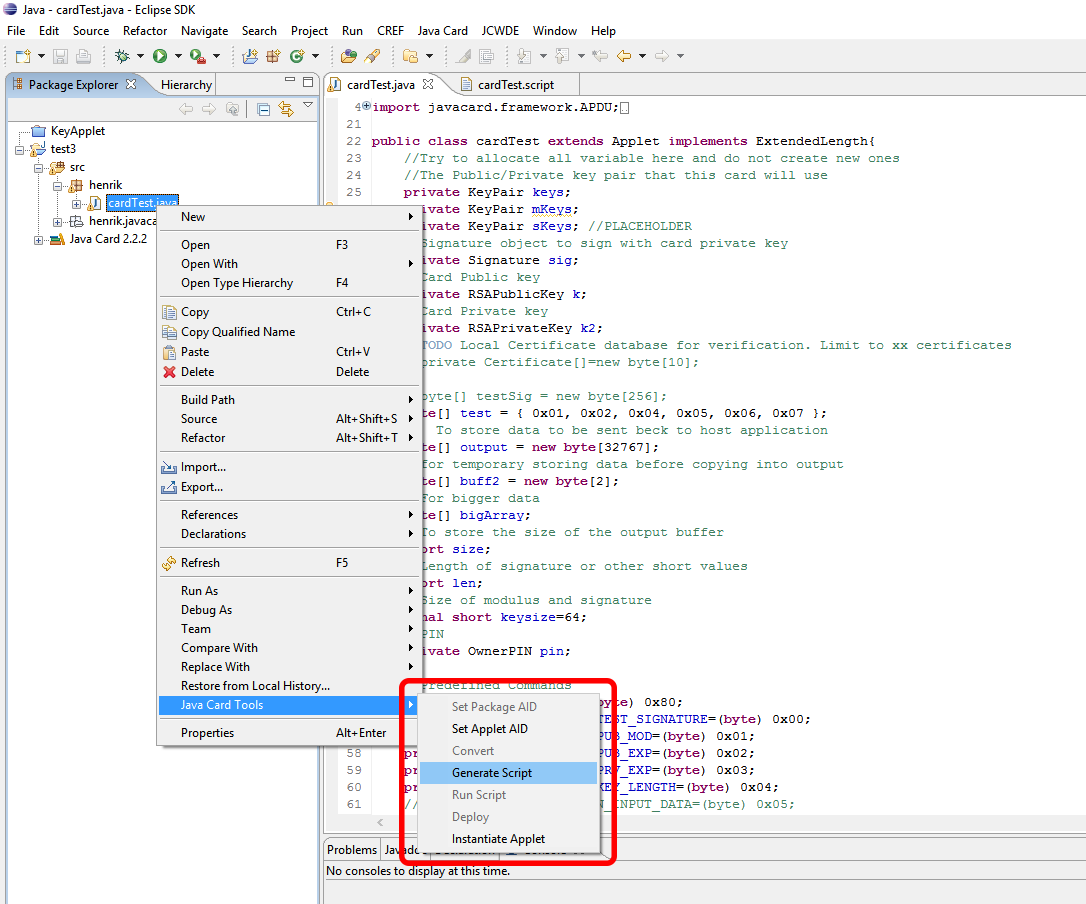
\includegraphics[width=0.95\textwidth]{images/eclipse.png}
\end{figure}

In figure \ref{fig:eclipse} we can see the tools for generating the deployable smart card application package. The screenshot also shows how the editor looks like any other Eclipse version. Even though this version of Eclipse includes tools for sending and receiving APDUs to the application (testing), we have decided not to use these tools as they proved themselves to be unstable and not representative of real world use. This is mostly due to the fact that the application is deployed to an emulator and does not have \textit{any} hardware limitations of a physical smart card.

\subsection{Deployment}
We will be using GlobalPlatformPro (GP) \cite{globalplatform} to deploy and manage applets on the physical smart cards. GP is a command line tool and is compatible with our hybrid Gemalto card with reader as well as the micro SD card. There are three essential steps when deploying an application to a smart card:

\begin{itemize}
    \item Delete the smart card application along with the stored data.
    \item Delete the smart card package.
    \item Install the new smart card.
\end{itemize}

To do this we will utilize a simple batch script which consisting of three lines of code (listing \ref{lst:batchInstall}). To gain access to the cards we need to provide a key set by the manufacturer. This requirement is added as an added security measure to verify that developers are supposed to have write access to the smart cards. Lastly we supply the AID we wish to use for our application. It is important to note that the AID must be unique and the installation will not succeed if the AID is in use.

\begin{lstlisting}[language=batch,caption=Install and deploy script for GlobalPlatformPro., label=lst:batchInstall,escapechar=!]
    gp.exe -visa2 -key !\%!KEY!\%! -delete !\%!AID!\%!
    gp.exe -visa2 -key !\%!KEY!\%! -delete !\%!PACKAGEID!\%!
    gp.exe -visa2 -key !\%!KEY!\%! -install !\%!PATH!\%! -d
\end{lstlisting}

\subsection{Basic testing environment}
To test the smart card application that is deployed on the physical cards (without going through an Android application) we will be using pyApduTool \cite{pyapdutool}. pyApduTool is a tool for sending APDUs to a smart card through a card reader or memory card reader and lets us observe how the card behave when receiving and transmitting data.

\begin{figure}[h!]
  \caption{Select APDU sent to smart card via PyApduTool}
  \label{fig:pyapdutool}
  \centering
    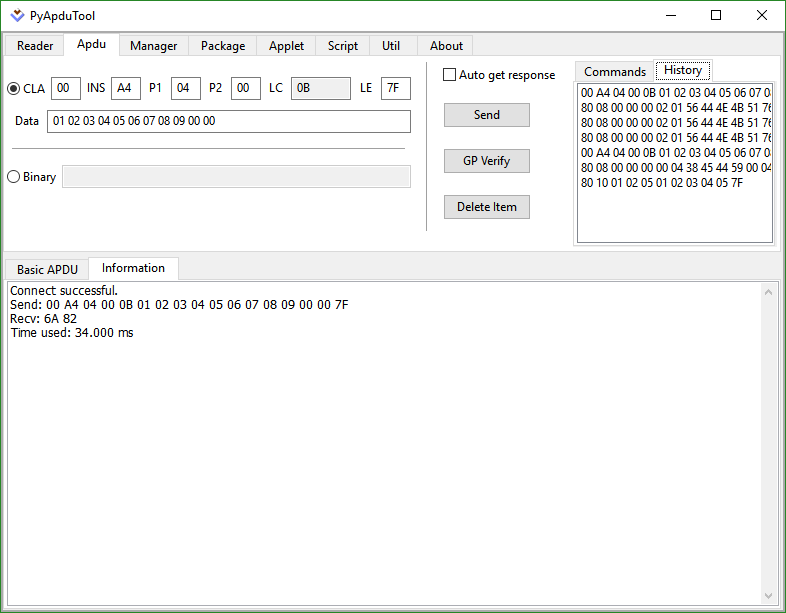
\includegraphics[width=0.95\textwidth]{images/pyapdutool.png}
\end{figure}

PyApduTool does not support extended APDU and this limits us to a high degree when testing our smart card application. Testing through PyApduTool does not test mobile device behaviour such as out of memory, too much traffic or NFC limitations. After the initial basic testing PyApduTool became obsolete and we had to test via an Android application.

\subsection{Application}
\paragraph{Goal}\mbox{}\\
The goal of the smart card application was to create an autonomous and easy to extend platform for future tests. This resulted in an application split into three parts.

\paragraph{Initialization}\mbox{}\\
As described in section \ref{sec:javacard} all javacard applications must implement the method \texttt{Install}. \texttt{Install} invokes the constructor of the smart card and this is where all variables that need initialization are initialized. For instance if the smart card application needs to generate keys or random numbers this is where it is done as the constructor will be invoked only once. All buffers that needs to be used should also be initialized here to avoid allocating memory everytime the application is used.

\paragraph{Data processing}\mbox{}\\
In the mandatory \texttt{Process} method (refer to section \ref{sec:javacard}) all data processing takes place. First a built in method in the javacard API, \texttt{selectingApplet()}, is invoked. This method checks if the incoming APDU is a SELECT APDU and acts accordingly. If the incoming APDU is not a SELECT APDU the incoming APDU is copied to a new buffer for easier data manipulation. Next we use a switch statement switching over the second byte, INS, to determine which instruction we want to perform. After processing the data and performing the work we want to do (sign data, encrypt, etc.) we copy our response to the outgoing buffer.

\paragraph{Finalization}\mbox{}\\
At the end of the \texttt{Process} invokation we invoke the \texttt{Send} method which takes the data in the outgoing buffer, package it for sending and send it as a response APDU.

\paragraph{The result}\mbox{}\\
What we end up with is a test plattform where we are only concerned with declaring variables, initializing variables and writing code for the specific test case. Listing \ref{lst:pseudoCard} shows pseudocode for the java card application with the extendable areas highlighted.


\begin{lstlisting}[caption=Pseudo code for javacard test application., label=lst:pseudoCard,escapechar=!]
public class cardApplication extends Applet implements ExtendedLength{

    !\colorbox{highlight}{//Variable declarations}!

    private cardApplication() {
    	!\colorbox{highlight}{//Variable initialization}!
    }

    public void process(APDU apdu) {
    	//Process incoming APDU
        if (selectingApplet()) {
			return;
		}
        buff = apdu.getBuffer();

    	switch(buff[ISO7816.OFFSET_INS]){
            case 0x00:
            case 0x01:
            !\colorbox{highlight}{...}!
            case 0xff:
            default:

    	}
    	Send(apdu);
    }

    private void send(APDU apdu) {
    	//Package outgoing buffer
    	//Send response APDU
    }
}
\end{lstlisting}

As seen in \ref{lst:pseudoCard} we allow for 256 cases/uses of the smart card, but if we include the use of P1 and P2 from section \ref{sec:communicationstandard} there are in theory 256\textsuperscript{3} = 16777216 possible cases. This does not include the pre-implemented methods which are explained in section \ref{sec:androidApp}. Their counterparts in the smart card application have the following byte values:

\begin{itemize}
    \item byte SEND\_U\_PUB\_MOD = (byte) 0x01;
    \item byte SEND\_U\_PUB\_EXP = (byte) 0x02;
    \item byte SIGN = (byte) 0x03;
    \item byte BINDING = (byte) 0x05;
    \item byte RSACRYPTO = (byte) 0x06;
    \item byte AESCRYPTO = (byte) 0x09;
\end{itemize}

We will not go into detail on how the individual cases are built up. Refer to Appendix A for JavaCard code.

\section{Android application}
\subsection{IDE}
Android Studio \cite{androidIDE} is the official IDE for Android application development. Android Studio is based on IntelliJ IDEA \cite{intelliJIDEA} and provides many automated tools for building, packaging and publishing Android applications.
\subsection{3rd party libraries}
As mentioned in section \ref{sec:equipment} Gemalto provides a java library, IDGo800, for using their smart cards.

\begin{aquote}{Gemalto.com \cite{GemaltoIDGo800}}
"IDGo 800 for Mobiles is a cryptographic middleware that supports the Gemalto IDPrime cards and Secure Elements on Mobile platforms: Contact and contactless smart cards, MicroSD cards, UICC-SIM cards, embedded Secure Elements (eSE) and Trusted Execution Environment (TEE)."
\end{aquote}

The part of IDGo800 SDK we are interested in is very small and enables us to send custom APDUs to micro SD smart cards.

We will be using the "android.nfc" package in order to communicate with NFC smart cards. This package is included in the standard Android SDK which in turns means that all Android devices with a NFC reader and minimum API level 9 \cite{androidNFCminSDK} can use our library.

\subsection{Application}
\label{sec:androidApp}

In section \ref{sec:designAndroidGoals} we described the goals of the framework. The first goal we will describe the implementation of is "extendable" or in other words, being able to send custom APDUs. Explaining how this is implemented will give a better understanding of how the framework is built up and makes it easier to understand the pre-implemented methods.

We used the same approach on the Android application as on the smart card application; an autonomous and easy to extend plattform for tests. This resulted in a new library, "smartcardlibrary",  which sole purpose is to transmit APDUs as easily as possible along with some basic functionality.

\paragraph{Custom APDUs}\mbox{}\\
To send custom APDUs to a smart card,\texttt{CommunicationController} must be instantiated and the application must know the application identifier of the smart card application. Further the current activity must implement\\ \texttt{NfCSmartcardControllerInterface} or \texttt{MSDSmartcardControllerInterface} (depending on smart card type) in order to be notified when the transaction is complete. Before continuing one will need to call the methods \texttt{setupNFCController} or \texttt{setupmSDController} depending on the smart card. Listing \ref{lst:NFCLibraryExample} shows an example implementation on how an activity may utilize the library for sending custom commands to a NFC smart card.

\begin{lstlisting}[caption=Java code example showing how to send and receive commands to a NFC smart card., label=lst:NFCLibraryExample,escapechar=å]

public class PayloadActivity extends AppCompatActivity
    implements NFCSmartcardControllerInterface {
    CommunicationController cc = new CommunicationController();
    ...

    private void initNFCCommunication(){


        String AID = "0102030405060708090007";
        String hexMessage = "95404F3FB1";
        String INS = "06";
        String p1 = "00";
        String p2 = "00";
        cc.setupNFCController(this, this);
        cc.initNFCCommunication(AID, INS, p1, p2, hexMessage);
    }

    å@Overrideå
    public void nfcCallback(final String completionStatus){
        if(!completionStatus.equals("OK")){
            return;
        }
        StorageHandler stHandler =
            new StorageHandler(getApplicationContext());
        String response =
            stHandler.readFromFileAppDir(
                FilePaths.tempStorageFileName
            );
    }
}

\end{lstlisting}

In order for the library to perform an asyncronous transaction the library will temporary save the responses from the cards to a file only accessible by the running application. To retrive the data the current activity should use the included \texttt{StorageHandler} class as used in listing \ref{lst:NFCLibraryExample}. The library also provides the class, \texttt{Converter}, for converting between Strings, hex and byte arrays.

\paragraph{Pre-implemented methods}\mbox{}\\
Recall the areas we want to cover from the beginning of the chapter. The functionality we have implemented so far are:

\begin{itemize}
    \item Bind smart card to mobile device.
    \item Encrypt/decrypt data using RSA key on card.
    \item Encrypt/decrypt data using AES key on card.
    \item Get public key of the smart card.
    \item Sign data using the public key of the smart card.
\end{itemize}

To use these functionalities one would only need to create an Android \texttt{Activity}, invoke either \texttt{setupNFCController(...)} or \texttt{setupmSDController(...)} (depending on smart card), and utilize the desired methods.
The methods available are:

\begin{itemize}
    \item public void disableNFC(...)
    \item public void bindingStepOne(...)
    \item public void bindingStepTwo(...)
    \item public void bindingStepThree(...)
    \item public void signData(...)
    \item public void cryptoRSA(...)
    \item public void cryptoAES(...)
    \item public void getCardPubMod(...)
    \item public void getCardPubExp(...)
\end{itemize}
The binding process is designed in three steps. First step is to ask the smart card if it requires a PIN-code and how many attempts are left. Second step requires a PIN-code and if this is correct the smart card application will move on to step three. The last step is sending the public key of the mobile device and getting the verification package from section \ref{sec:proposedSolution}. More discussion on this matter in section \ref{sec:bindingcardandphone}.

The rest of the methods should be self-explanatory and one should refer to the javadoc in Appendix A for parameter requirements and pre-conditions.

Figure \ref{fig:package} shows how the library is structured and the entry point for applications is through the packages:

\begin{itemize}
    \item com.master.henrik.controller
    \item com.master.henrik.statics
    \item com.master.henrik.shared
\end{itemize}

%TODO UPDATE

\begin{figure}[h!]
  \caption{Library package diagram.}
  \label{fig:package}
  \centering
    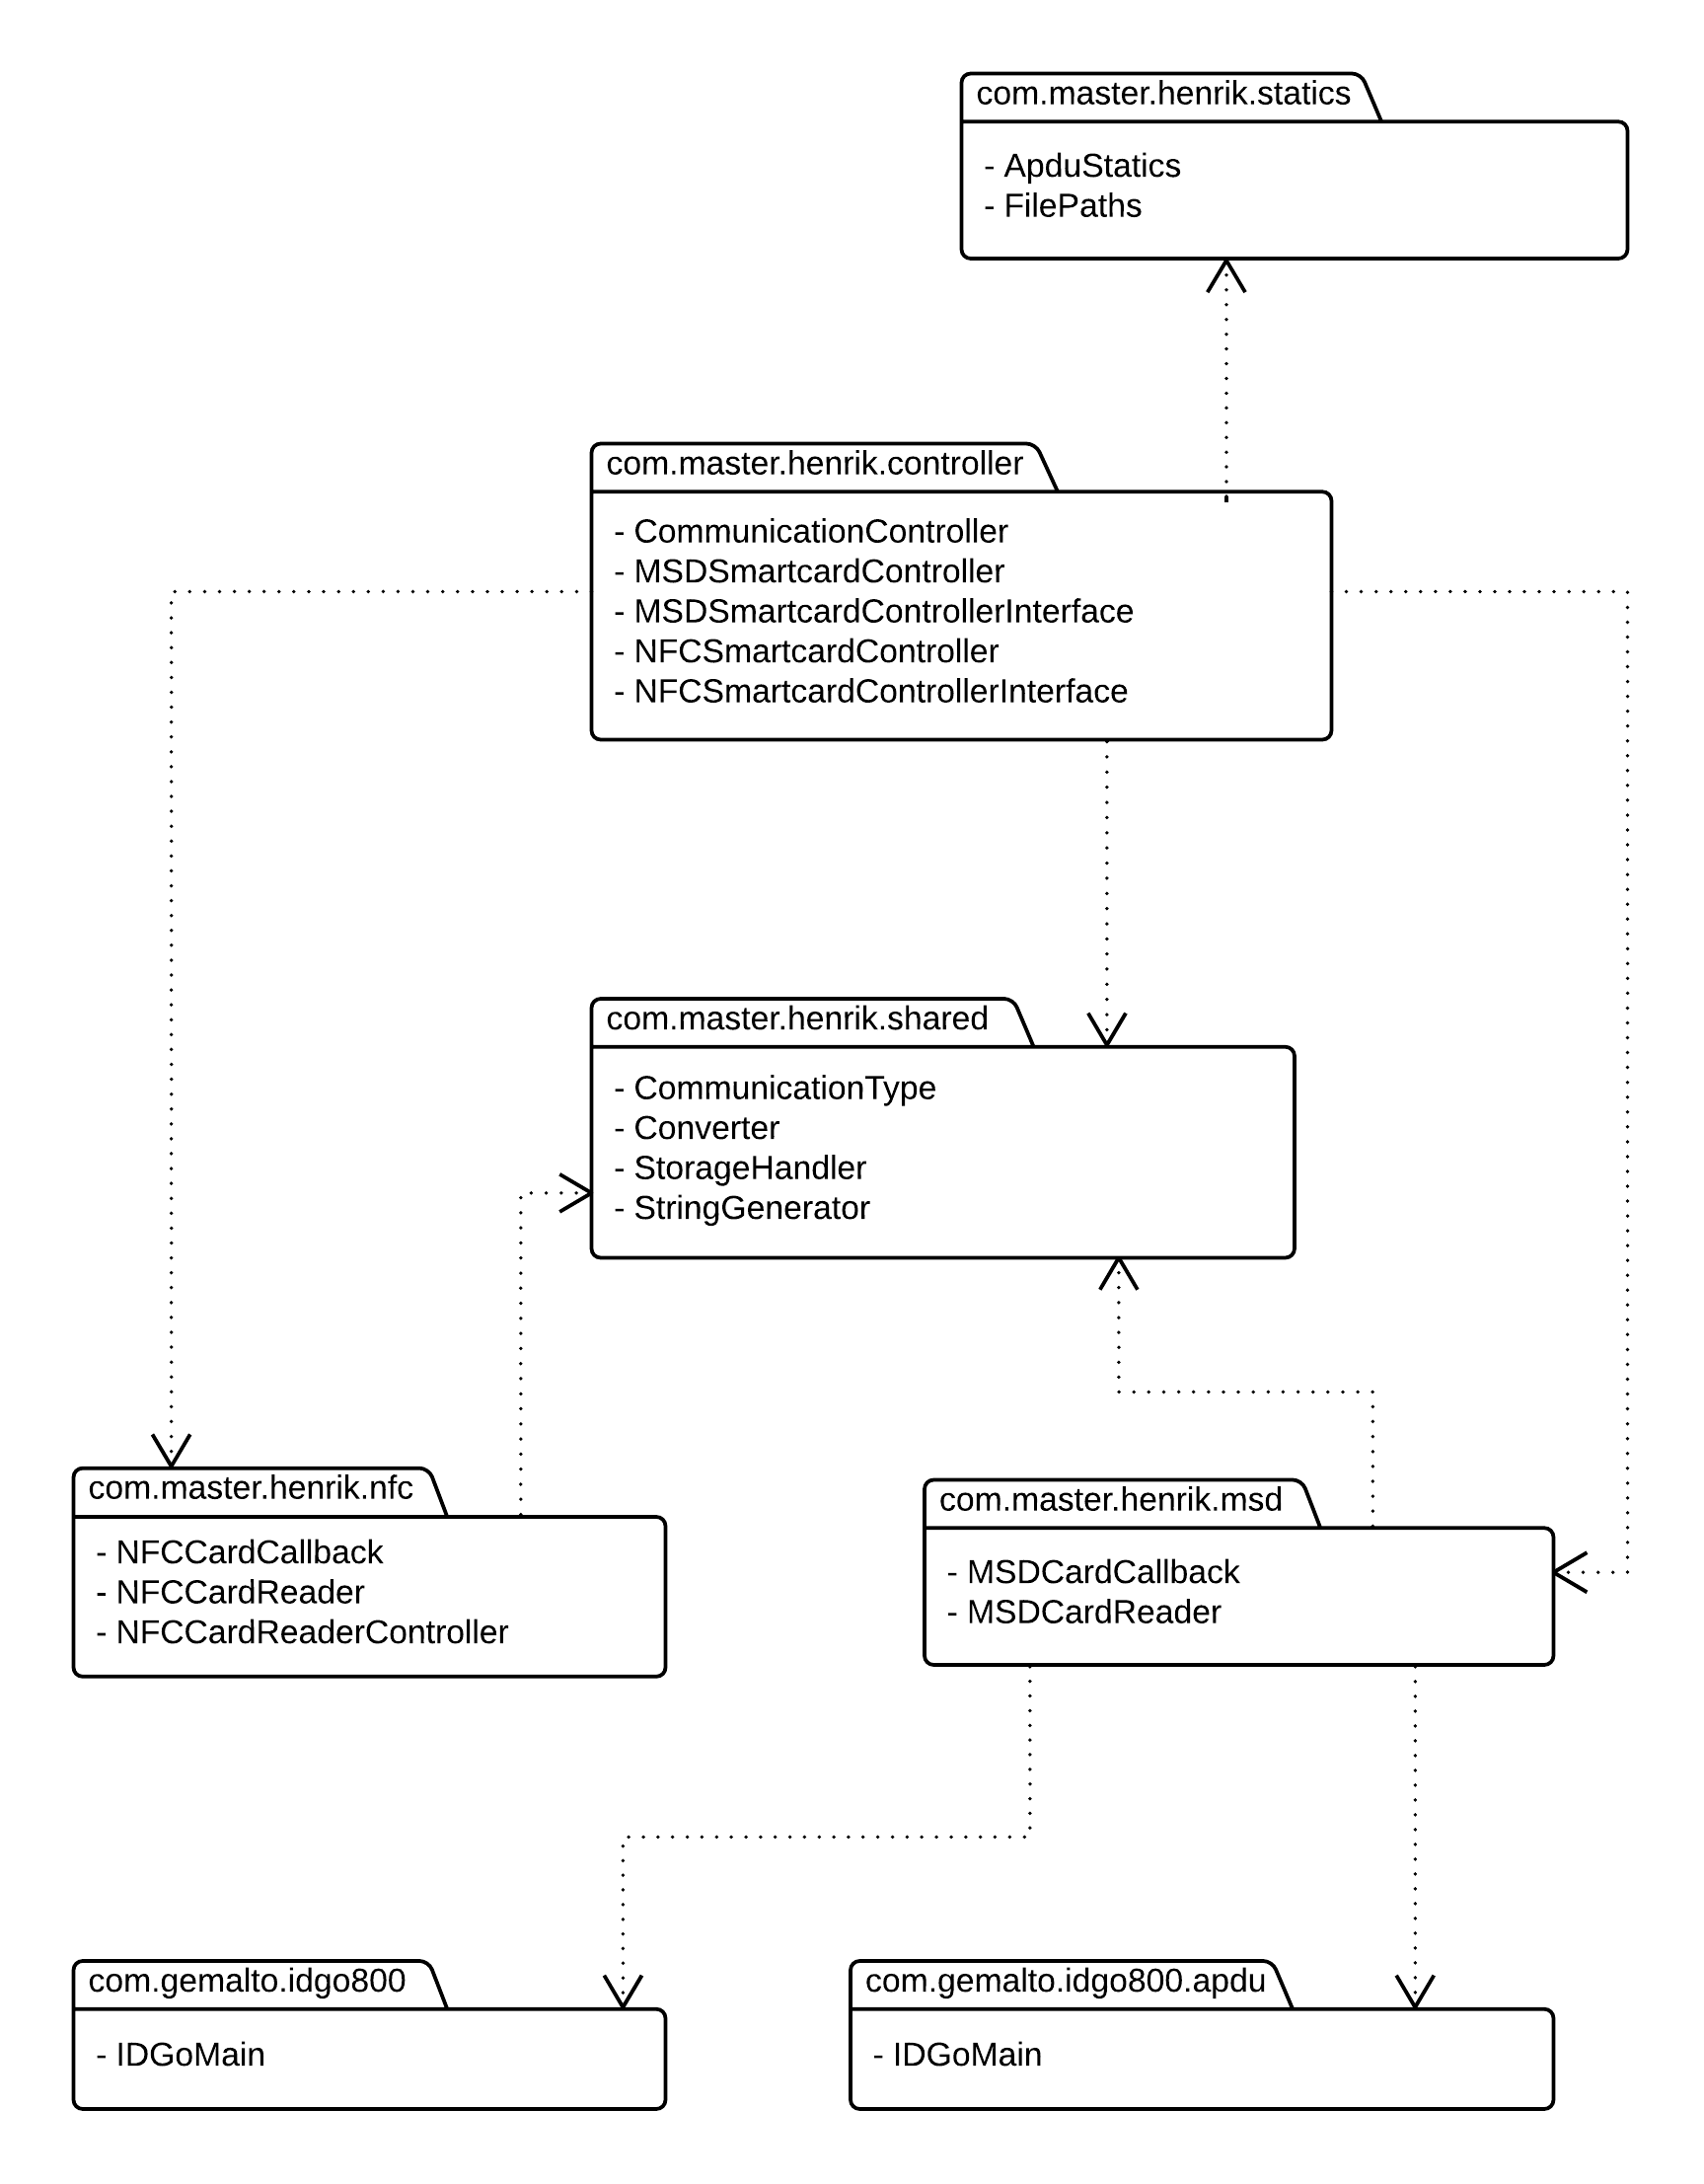
\includegraphics[width=0.95\textwidth]{images/package2.png}
\end{figure}
